\documentclass[13.5pt,aspecratio=169]{beamer}
\usepackage{graphicx} % Required for inserting images
\usepackage{amsfonts}
\usepackage{amsmath}
\usepackage{amssymb}
\usepackage{physics}
\usepackage{bm}
\usepackage{physics}
\usepackage{booktabs}
\usetheme{Madrid}

\DeclareMathOperator*{\argmax}{arg\,max}
\DeclareMathOperator*{\argmin}{arg\,min}
\graphicspath{{Images/}{./}} 
\usetheme{Copenhagen}
%\usecolortheme{beaver}
\title{CHAPTER 5: Logistic Regression}
\author[Group 5]{\textit{Instructor: PhD. Nguyen Thi Quy}\\ \bigskip \textbf{Group 5: 5.4 - 5.6.1}}
\date{\today}
\setbeamertemplate{navigation symbols}{}
\setbeamertemplate{headline}{}
\setbeamercolor{huge text}{fg=white}
%\setbeamercovered{transparent}
\setbeamertemplate{footline}{
    \leavevmode%
    \hbox{%
        \begin{beamercolorbox}[wd=.333333\paperwidth,ht=2.25ex,dp=1ex,center]{author in head/foot}%
            \usebeamerfont{author in head/foot}\insertshortauthor
        \end{beamercolorbox}%
        \begin{beamercolorbox}[wd=.333333\paperwidth,ht=2.25ex,dp=1ex,center]{title in head/foot}%
            \usebeamerfont{title in head/foot}\insertshorttitle
        \end{beamercolorbox}%
        \begin{beamercolorbox}[wd=.333333\paperwidth,ht=2.25ex,dp=1ex,right]{date in head/foot}%
            \usebeamerfont{date in head/foot}\insertshortdate{}\hspace*{2em}
            \insertframenumber{} / \inserttotalframenumber\hspace*{2ex} 
        \end{beamercolorbox}%
    }%
    \vskip0pt%
}

\begin{document}
\maketitle

% \begin{frame}
% 	\frametitle{Table of Contents} % Slide title, remove this command for no title
% 	\tableofcontents[subsectionstyle=hide]
% \end{frame}
%-------------------------------------------------------------------%

\section{5.4: Learning in Logistic Regression}
% \begin{frame}
% 	\frametitle{Table of Contents} % Slide title, remove this command for no title
% 	\tableofcontents[currentsection, subsectionstyle=hide]
% \end{frame}

\begin{frame}
    \bigskip
    \color{blue} \Huge \textbf{5.4 Learning in Logistic Regression} 
\end{frame}

%-------------------------------------------------------------------%
\begin{frame}
    \frametitle{{Learning in Logistic Regression}}
    \only <1,2> {\begin{block}{Supervised classification:}
        \begin{itemize}
            \item We know the correct label \color{blue} y \color{black} (either 0 or 1) for each x. 
            \item But what the system produces is an estimate, \color{blue} $\hat{y}$ \color{black} .
        \end{itemize}
    \end{block}}
    \bigskip
    \only<2>{ We want to set w and b to minimize the distance between our estimate $y^i$ and the true $\hat{y}^i$.  
        \begin{itemize}
            \item We need a distance estimator: \textbf{a loss function} or \textbf{a cost function}
            \item  We need \textbf{an optimization algorithm} to update w and b to minimize the loss.
        \end{itemize}
    }
    \only <3> {
        \begin{block}{\Large Learning components:}
            \begin{itemize}
                \item A loss function: \textbf{cross-entropy loss}.
                \item An optimization algorithm: \textbf{stochastic gradient descent}.
            \end{itemize}
        \end{block}
    }
\end{frame}
%-------------------------------------------------------------------%

\section{5.5 The cross-entropy loss function}

% \begin{frame}{Tables of contents}
%     \tableofcontents[currentsection]
% \end{frame}
\begin{frame}
    \bigskip
    \color{blue} \Huge \textbf{5.5 The cross-entropy loss function} 
\end{frame}

%-------------------------------------------------------------------%
\begin{frame}
    \frametitle{The cross-entropy loss function}
    {\Large The distance between $\hat{y}$ and y}
    \bigskip
    \begin{block}{We want to know how far is the classifier output:}
        {\hphantom{xyz}  $\hat{y} = \sigma(w.x+b)$ }

    \end{block}

    \begin{block}{From the true output:}
        {\hphantom{xyz} y     [ = either 0 or 1]} 
    \end{block}
    \onslide<2>\begin{block}{ We'll call this difference:}
        $=>$ L($\hat{y}$,y) = how much $\hat{y}$ differs from the true y 
    \end{block}
\end{frame}
%-------------------------------------------------------------------%
\begin{frame}{Cross-entropy loss}
    \begin{block}{\Large Conditional maximum likelihood estimation}
        We choose the parameters w,b that: 
        \begin{itemize}
            \item \textbf{maximize} the log probability 
            \item of the \textbf{true y labels} in the training data 
            \item  given the observations x
        \end{itemize}
    \end{block}
    \begin{exampleblock}{}
         The resulting loss function is the \textbf{ negative log likelihood loss}, generally called the \textbf{cross-entropy loss}.
    \end{exampleblock}
\end{frame}
%-------------------------------------------------------------------%
\begin{frame}{Cross-entropy loss}
    \begin{block}{\large \textbf{Goal: maximize probability of the correct label p(y$|$x) }}
        Since there are only 2 discrete outcomes (0 or 1) we can express the probability $p(y|x)$ from our classifier (the thing we want to maximize) as:
        \centerline{$p(y|x) = \hat{y}^{y} (1-\hat{y})^{1-y} \hspace{20} \color{blue} (1) \color{black}$} 
        NOTE:
        \begin{itemize}
            \item if y=1, this simplifies to $\hat{y}$
            \item if y=0, this simplifies to $1 - \hat{y}$
        \end{itemize}
    \end{block}
\end{frame}
%-------------------------------------------------------------------%
\begin{frame}{Cross-entropy loss}
    \frametitle{The cross-entropy loss function}
    \begin{exampleblock}{}
        \textbf{Goal}: maximize probability of the correct label p(y$|$x) 
    \end{exampleblock}

    \bigskip

    Maximize: \hphantom{xyzxyz}{$p(y|x) = \hat{y}^{y} (1-\hat{y})^{1-y} \hspace{20} \color{blue} (1) \color{blacl}$}
    
    \bigskip

    \begin{exampleblock}{}
        Take the log of both sides:
    \end{exampleblock}

    \bigskip

    Maximize: \hphantom{xyzxyz} $\log{p(y|x)} &= \log{[\hat{y}^{y} (1-\hat{y})^{1-y}]} \\
    \hphantom{Maximize: xyzxyz  \log{p(y|x)} } &= y \log{\hat{y}}+(1-y)\log{(1-\hat{y})} \hspace{10}\color{blue} (2) \color{black}$
\end{frame}
%-------------------------------------------------------------------%
\begin{frame}{Cross-entropy loss}
    \begin{block}{\large \textbf{Goal: maximize probability of the correct label p(y$|$x) }}
        \begin{itemize}
            \item  \textbf{Maximize}:  \log{p(y|x)}$= y \log{\hat{y}}+(1-y)\log{(1-\hat{y})} \hspace{10}\color{blue} (2) \color{black}$
            \item Flip sign to turn this into a loss: something to \textbf{minimize}
            \vskip .1cm
            \textbf{Minimize:}
            \hphantom{xyzxyz} {$L_{CE} (\hat{y},y) = - \log{p(y|x)} = - [y \log{\hat{y}}+(1-y)\log{(1-\hat{y})}]\color{blue} (3) \color{black}$}               
        \end{itemize}
    \end{block}
    \begin{block}{\textbf{Plugging in definition of y ̂: {$\hat{y} = \sigma(w.x+b)$ }}}
        \centerline{$L_{CE} (\hat{y},y) = - [y \log{\sigma(w.x+b) }+(1-y)\log{(1-\sigma(w.x+b))}]\color{blue} (4) \color{black}$}     
    \end{block}
\end{frame}
%-------------------------------------------------------------------%
\begin{frame}{Cross-entropy loss}
    \begin{block}{\textbf{Plugging in definition of y ̂: {$\hat{y} = \sigma(w.x+b)$ }}}
        \centerline{$L_{CE} (\hat{y},y) = - [y \log{\sigma(w.x+b) }+(1-y)\log{(1-\sigma(w.x+b))}]\color{blue} (4) \color{black}$}     
    \end{block}
    \begin{block}{We want loss to be:}
        \begin{itemize}
            \item \textbf{Smaller} if the model estimate is close to correct
            \item \textbf{Bigger} if model is confused
        \end{itemize}
    \end{block}
\end{frame}
%-------------------------------------------------------------------%
\begin{frame}{Let's see if this works for our sentiment example}
    \begin{exampleblock}{Example: Fig 5.2}
        \vskip \hspace{10} It's hokey. There are virtually no surprises, and the writing is second-rate.         So why was it so enjoyable ? For one thing, the cast is great. Another nice touch is the music. I was overcome with the urge to get off the couch and start dancing. It sucked me in, and it'll do the same to you.
    \end{exampleblock}
    \begin{exampleblock}{With:}
        $ w = [2.5,−5.0,−1.2,0.5,2.0,0.7], b = 0.1, x = [3,2,1,3,0,4.19]$
    \end{exampleblock}
\end{frame}
%-------------------------------------------------------------------%
\begin{frame}{Fig 5.2}
    \begin{exampleblock}{Check:}
        $L_{CE} (\hat{y},y) = - [y \log{\sigma(w.x+b) }+(1-y)\log{(1-\sigma(w.x+b))}]\color{blue} (4) \color{black}$ 
        \begin{itemize}

            \item  With:
            \centerline{$ w = [2.5,−5.0,−1.2,0.5,2.0,0.7], b = 0.1, x = [3,2,1,3,0,4.19]$}
        \end{itemize}
    \end{exampleblock}
    \begin{exampleblock}{Let's first suppose the true label of this is y=1 (positive)}
        \centerline{$L_{CE} (\hat{y},y) =  - y \log{\sigma(w.x+b) }$}
        \vskip
        \hspace{129}$= - \log{\sigma(w.x+b)}$
        \vskip
        \hspace{129}$= - \log{0.70}$
        \vskip
        \hspace{129}$= 0.36$
    \end{exampleblock}
\end{frame}
%-------------------------------------------------------------------%
\begin{frame}{Fig 5.2}
    \begin{exampleblock}{Check:}
        $L_{CE} (\hat{y},y) = - [y \log{\sigma(w.x+b) }+(1-y)\log{(1-\sigma(w.x+b))}]\color{blue} (4) \color{black}$ 
        \begin{itemize}
            \item  With:
            \centerline{$ w = [2.5,−5.0,−1.2,0.5,2.0,0.7], b = 0.1, x = [3,2,1,3,0,4.19]$}
        \end{itemize}
    \end{exampleblock}
    \begin{exampleblock}{Let's first suppose the true label of this is y=0 (negative)}
        \centerline{$L_{CE} (\hat{y},y) =  - (1-y)\log{(1-\sigma(w.x+b)) }$}
        \\
        \hspace{102}$= - \log{1-\sigma(w.x+b)}$
        \\
        \hspace{102}$= - \log{0.30}$
        \\
        \hspace{102}$= 1.2$
    \end{exampleblock}
\end{frame}
%-------------------------------------------------------------------%
\begin{frame}{Let’s see if this works for our sentiment example}
    \begin{block}{}
         \begin{itemize}
           \item  The loss when model was right (if true y=1):
           \centerline{$L_{CE}(\hat{y},y) = 0.36$}
           \item Is lower than the loss when model was wrong (if true y=0):
            \centerline{$L_{CE} (\hat{y},y) = 1.2$}
        \end{itemize}
    \end{block}
    \Large \textbf{Sure enough, loss was bigger when model was wrong!
}
\end{frame}
%-------------------------------------------------------------------%

\section{5.6: Gradient Descent} % Sections are added in order to organize your presentation into discrete blocks, all sections and subsections are automatically output to the table of contents as an overview of the talk but NOT output in the presentation as separate slides
% \begin{frame}
% 	\frametitle{Presentation Overview} % Slide title, remove this command for no title
% 	\tableofcontents[currentsection, subsectionstyle=hide]
% \end{frame}

\begin{frame}
    \bigskip
    \color{blue} \Huge \textbf{5.6: Gradient Descent} 
\end{frame}

%------------------------------------------------

\begin{frame}
	\frametitle{Gradient Descent}
	\begin{block}{} % Block without title
		\textbf{Our goal:} minimize the loss.
	\end{block}
    
    \begin{block}{} % Block without title
        Let's make explicit that the loss function is parameterized by weights $\theta = (w,b)$
	\end{block}
    \begin{itemize}
        \item And we'll represent $\hat{y}$ as \textit{$f(x; \theta)$} to make the dependence on $\theta$ more obvious.
	\end{itemize}

    \begin{block}{} % Block without title
        We want the weights that minimize the loss, averaged over all examples:
	\end{block}
    {\fontsize{16}{20}\selectfont
    \begin{center} % Centering the equation
        \[ \bm{\hat{\theta}} =  \underset{\bm{\theta}}{\text{argmin}} \frac{\bm{1}}{\bm{m}} \sum_{i=1}^{m} \bm{\mathcal{L}}_{\bm{CE}}(f(x^{(i)}; \bm{\theta}), y^{(i)})\]
      \end{center}
    }

\end{frame}
%------------------------------------------------



\subsection{Intuition of gradient descent}

\begin{frame}
\onehalfspacing
	\frametitle{Intuition of gradient descent}
	
	\begin{block}{} % Block without title
		How do I get to the bottom of this river canyon?
	\end{block}
        \bigskip
        \begin{figure}[h]
            \begin{minipage}{0.5\textwidth} % Adjust the width as needed
                \centering
                
\includegraphics[scale=0.4]{river_canyon.png} % Replace with your image file
            \end{minipage}
            \hfill
            \begin{minipage}{0.45\textwidth} % Adjust the width as needed
                Look around me $360^\circ$ \\
                Find the direction of steepest slope down \\
                Go that way 
            \end{minipage}
        \end{figure}
\end{frame}


%------------------------------------------------
\begin{frame}
\onehalfspacing
	\frametitle{Our goal: minimize the loss}
    \begin{block}{} % Block without title
		For logistic regression, loss function is convex
	\end{block}
	    \begin{itemize}
		    \item A convex function has just one minimum
                \item Gradient descent starting from any point is
                guaranteed to find the minimum

                
                \begin{itemize}
                   
                            \item (Loss for neural networks is non-convex)
                                                
                \end{itemize}
		\end{itemize}
        \begin{figure}[h]
            \centering
            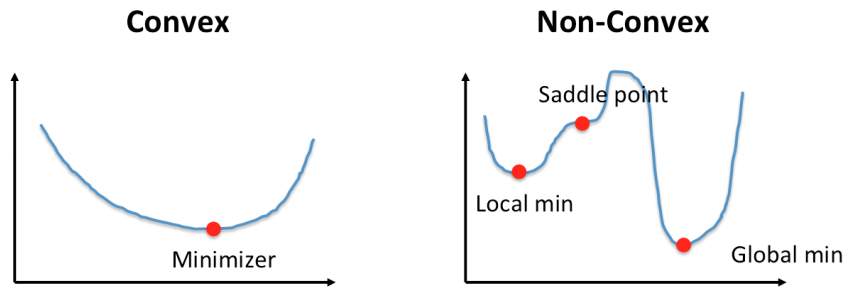
\includegraphics[scale=0.5]{convex.png}
        \end{figure}
\end{frame}


%------------------------------------------------


\begin{frame}
\onehalfspacing
	\frametitle{Our goal: minimize the loss}
	{\Large Let's first visualize for a single scalar w}
	\begin{block}{}
		\textbf{Q}: Given current w, should we make it bigger or smaller? \\
        \textbf{A}: Move w in the reverse direction from the slope of the functio
	\end{block}
	\bigskip
        \begin{figure}
            \centering
            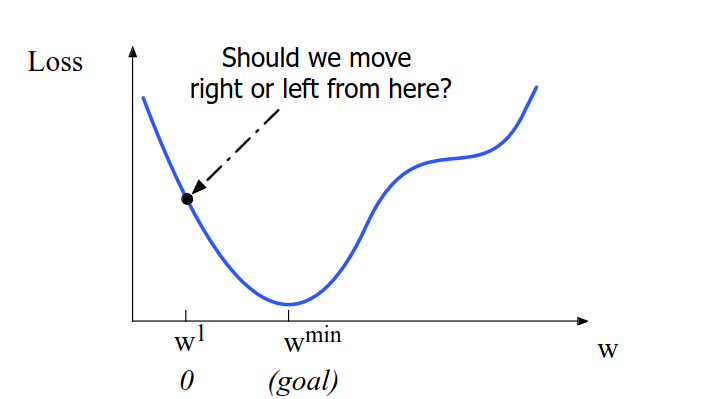
\includegraphics [scale=0.45] {visualize_0.png}
            
            \label{fig:enter-label}
        \end{figure}
	
\end{frame}
%------------------------------------------------


\begin{frame}
    \onehalfspacing
        \frametitle{Our goal: minimize the loss}
        {\Large Let's first visualize for a single scalar w}
        \begin{block}{}
            \textbf{Q}: Given current w, should we make it bigger or smaller? \\
            \textbf{A}: Move w in the reverse direction from the slope of the functio
        \end{block}
        \bigskip
            \begin{figure}
                \centering
                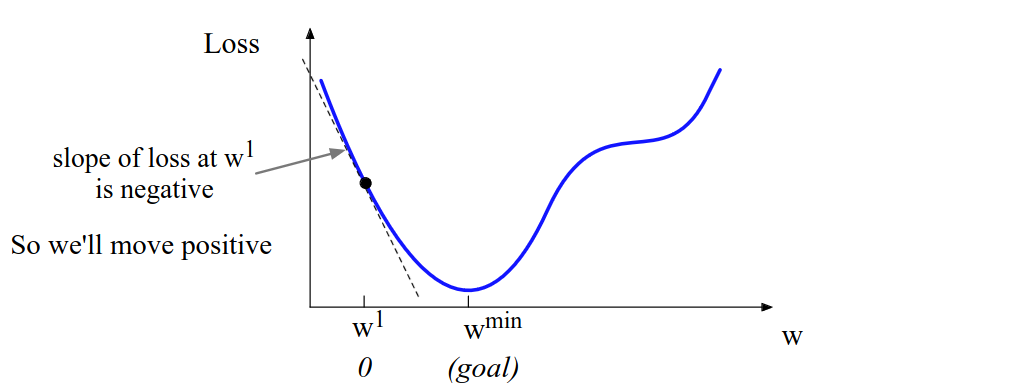
\includegraphics [scale=0.45] {visualize_1.png}
                
            \end{figure}
        
    \end{frame}
%------------------------------------------------

\begin{frame}
    \onehalfspacing
        \frametitle{Our goal: minimize the loss}
        {\Large Let's first visualize for a single scalar w}
        \begin{block}{}
            \textbf{Q}: Given current w, should we make it bigger or smaller? \\
            \textbf{A}: Move w in the reverse direction from the slope of the functio
        \end{block}
        \bigskip
            \begin{figure}
                \centering
                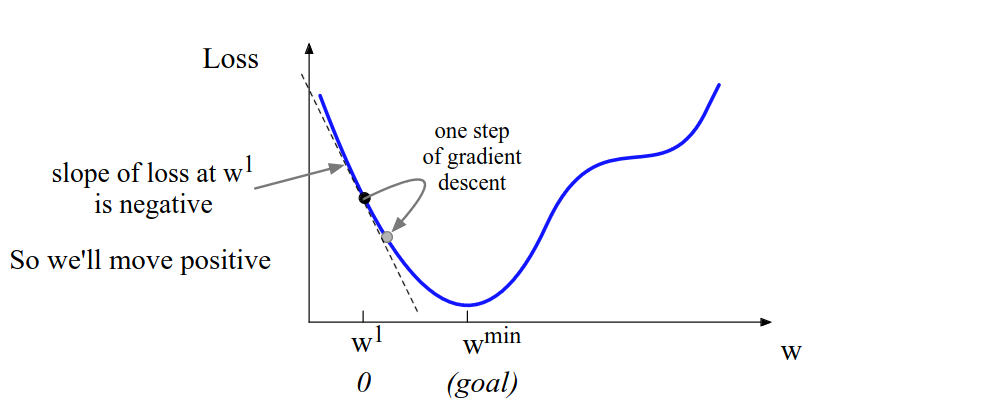
\includegraphics [scale=0.45] {visualize_2.png}
                
            \end{figure}
        
    \end{frame}
%------------------------------------------------
\begin{frame}
\onehalfspacing
	\frametitle{Gradients}
    \begin{block}{}
        The \textbf{gradient} of a function of many variables is a
vector pointing in the direction of the greatest
increase in a function.
    \end{block}

	\bigskip

    \begin{block}{}
        \textbf{Gradient Descent}: Find the gradient of the loss
function at the current point and move in the
\textbf{opposite} direction.
    \end{block}
\end{frame}

%------------------------------------------------
\begin{frame}
\onehalfspacing
	\frametitle{Gradient Descent Concepts}
    {\Large How much do we move in that direction ?}
    \bigskip
    \begin{itemize}
        \item The value of the gradient (slope in our example) \\ $ \dv{w} \mathcal{L} (f(x; w), y) $ weighted by a learning rate $\eta$
        \smallskip
        \item Higher learning rate $\eta$ means move w faster
    \end{itemize}

    {\fontsize{16}{20}\selectfont
    \begin{center} % Centering the equation
        \[ w^{t+1} =  w^t - \eta \dv{w} \mathcal{L} (f(x; w), y) \]
      \end{center}
    }
\end{frame}

%------------------------------------------------
\onehalfspacing
\begin{frame} % Use [allowframebreaks] to allow automatic splitting across slides if the content is too long
	\frametitle{Reference}
	
	\begin{thebibliography}{99} % Beamer does not support BibTeX so references must be inserted manually as below, you may need to use multiple columns and/or reduce the font size further if you have many references
		\footnotesize % Reduce the font size in the bibliography
		
		\bibitem[Stanford]{p1}
			Speech and Language Processing (3rd ed. draft)
			\newblock Dan Jurafsky and James H. Martin
			\newblock Part I: Fundamental Algorithms, \emph{Chapter 5: 	Logistic Regression}
			
		
	\end{thebibliography}
\end{frame}



%	CLOSING SLIDE
%----------------------------------------------------------------------------------------

\begin{frame} % The optional argument 'plain' hides the headline and footline
	\begin{center}
		{\Huge Thanks for listening!}
		
		\bigskip\bigskip % Vertical whitespace
		
		{\LARGE Q\&A section}
	\end{center}
\end{frame}
%------------------------------------------------


\end{document}
